\documentclass[12pt]{article}
\usepackage[utf8]{inputenc}
\usepackage[margin=1in]{geometry}
\usepackage[spanish]{babel}\decimalpoint
\usepackage{setspace}\onehalfspacing
\usepackage{parskip} % Espacio entre parrafos.
\usepackage{graphicx} % Para usar comando \includegraphics[]{}
\usepackage{amssymb} % Para usar el simbolo del conj. de los Reales.
\usepackage{amsmath} % Para usar columnas vectoriales.
\usepackage{multirow} % Para unir multiples filas en una tabla.
\usepackage{hyperref} % Siempre debe ser el ultimo paquete.


\setcounter{tocdepth}{2} % Que no incluya subsubsections en la tabla de contenidos (toc).

%================================

\title{Clase 23. Aplicación de las Integrales: Valor Promedio y Probabilidades.}
\author{MIT 18.01: Single Variable Calculus.}
\date{}


\begin{document}

\maketitle

\begin{abstract}
\noindent Otra aplicación relevante de las integrales, es en el cálculo del valor promedio de un conjunto infinito de valores. A partir de aquel, veremos el promedio ponderado y la probabilidad de un evento interpretada a partir de este último.
\end{abstract}


\section{Valor Promedio.}

En la Clase 20 vimos parcialmente el valor promedio de una función y se encuentra muy vinculado a la definición de la integral definida.

Sea $f(x)$ una función continua en $a \leq x \leq b$, donde:
\[
  \frac{f(x_{1}) + f(x_{2}) + \cdots + f(x_{n})}{n} = \frac{1}{n} \cdot \sum_{i = 1}^{n} f(x_{i})
\]
Si $n \to \infty$, obtenemos el \textbf{valor promedio continuo} de $f(x)$:
\[
  \lim_{n \to \infty} \left(\frac{1}{n} \cdot \sum_{i = 1}^{n} f(x_{i}) \right) = \frac{1}{b - a} \cdot \int_{a}^{b} f(x)dx
\]
\textbf{Demostración.} La definición de la integral definida está dada por:
\[
  \lim_{n \to \infty} \left(\sum_{i = 1}^{n} f(x_{i})\Delta x\right) = \int_{a}^{b} f(x)dx
\]
donde $\Delta x$ es el ancho de los $n$ intervalos adentro de $[a, \ b]$.
\[
  \Delta x = \frac{b - a}{n}
\]
Multipliquemos a la definición de la integral por el recíproco del ancho de $[a, \ b]$.
\[
  \frac{1}{b - a} \cdot \lim_{n \to \infty} \left(\sum_{i = 1}^{n} f(x_{i})\Delta x\right) = \frac{1}{b - a} \cdot \int_{a}^{b} f(x)dx
\]
El lado izquierdo es equivalente a:
\[
  \lim_{n \to \infty} \left(\frac{1}{b - a} \cdot \sum_{i = 1}^{n} f(x_{i}) \Delta x\right) =
  \lim_{n \to \infty} \left(\sum_{i = 1}^{n} \left[\frac{1}{b - a} \cdot f(x_{i}) \Delta x \right]\right) 
\]
Y $\Delta x = (b - a)/n$. Por lo tanto:
\begin{align*}
  \lim_{n \to \infty} \left(\sum_{i = 1}^{n} \left[\frac{1}{b - a} \cdot f(x_{i}) \cdot \frac{b - a}{n}\right]\right) &=
  \frac{1}{b - a} \cdot \int_{a}^{b} f(x)dx \\
  \lim_{n \to \infty} \left(\sum_{i = 1}^{n} \frac{1}{n} \cdot f(x_{i})\right) &= \frac{1}{b - a} \cdot \int_{a}^{b} f(x)dx \\
  \lim_{n \to \infty} \left(\frac{1}{n} \cdot \sum_{i = 1}^{n} f(x_{i})\right) &= \frac{1}{b - a} \cdot \int_{a}^{b} f(x)dx \quad (\text{Q.E.D})
\end{align*}
La idea del valor promedio continuo es la misma a la del cálculo de la media aritmética: Sumamos un conjunto de valores numéricos y lo dividimos por su cantidad. No obstante, en el primero tenemos infinitos valores, por tanto tomamos un intervalo que los incluyan y, luego, calculamos el cociente entre la integral y el ancho de dicho intervalo.

La similitud entre la media aritmética y el valor promedio continuo podemos verlo al calcularlos usando una función continua. Por ejemplo, el promedio de $5$ valores de salida de $f(x) = c$ ($c =$ constante y $x \in \mathbb{R}$) es igual a $c$:
\[
  \frac{c + c + c + c + c}{5} = \frac{5c}{5} = c
\]
Lo mismo ocurre si calculamos el promedio de infinitos valores de salida de $f(x) = c$:
\[
  \frac{1}{b - a} \cdot \int_{a}^{b} cdx = \frac{1}{b - a} \cdot (b - a) \cdot c = c
\]

\subsection{Ambigüedad del Valor Promedio.}

El valor promedio siempre dependerá de la variable con la que lo estemos calculando. En otras palabras, según la medida que usemos obtendremos un resultado que será distinto para otra.

\textbf{Ejercicio 1.} Calcule la altura promedio de un semicírculo unitario positivo con respecto a $x$.

\textbf{Solución.} La ecuación del círclo unitario es $x^{2} + y^{2} = 1$ y, al despejar $y$, resulta en $y = \pm \sqrt{1 - x^{2}}$. Como estamos trabajando con la mitad positiva, usaremos $f(x) = \sqrt{1 - x^{2}}$, donde $y = f(x)$.

Lo siguiente es graficar la función $f(x) = \sqrt{1 - x^{2}}$, remarcando la variable con la que mediremos su altura promedio.

\begin{figure}[hbt!]
\centering
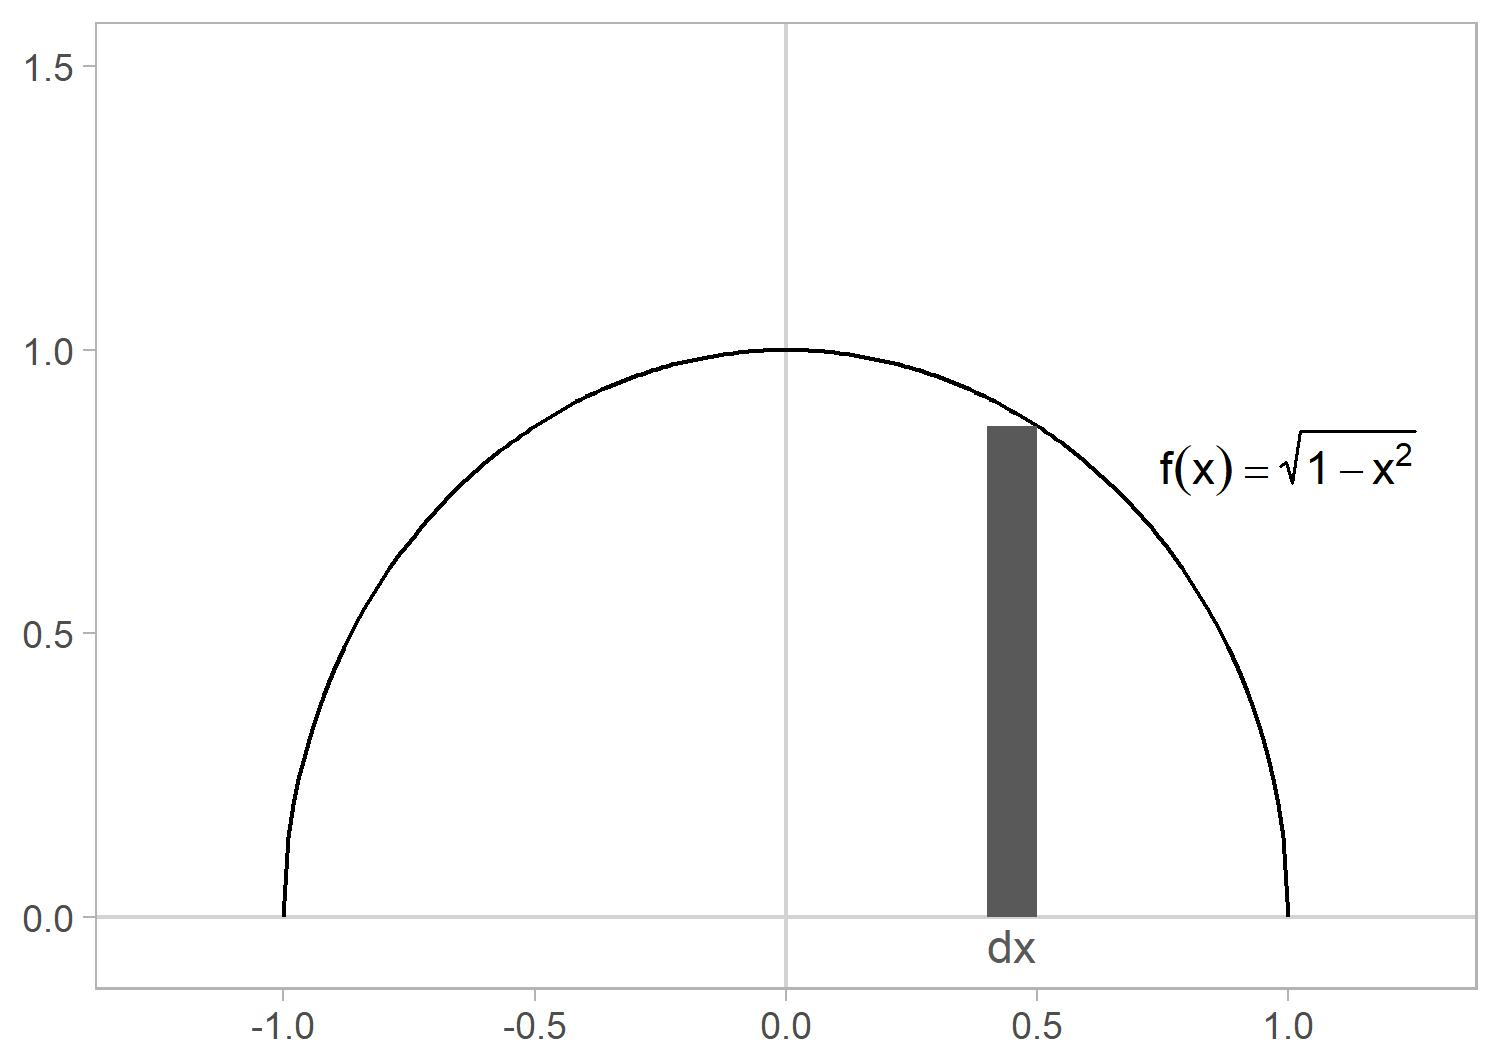
\includegraphics[scale=0.7]{img/avg-val-ex-1.jpg}
\end{figure}

Apliquemos la fórmula del valor promedio continuo para obtener la altura promedio del semicírculo, que denotaremos como $h_{p}$. Como la estamos calculando con respecto a $x$, entonces lo haremos adentro del intervalo $[-1, \ 1]$ (es unitaria).
\[
  h_{p} = \frac{1}{1 - (-1)} \cdot \int_{-1}^{1} \sqrt{1 - x^{2}}dx = \frac{1}{2} \cdot \int_{-1}^{1} \sqrt{1 - x^{2}}dx
\]
De momento no sabemos calcular la antiderivada\footnote{Necesitamos saber técnicas de integración, las cuales veremos en próximas clases.} de $\int_{-1}^{1} \sqrt{1 - x^{2}}dx$, pero podemos deducir que es el área del semicírculo, el cual es igual a $(\pi \cdot r^{2})/2$ donde $r$ es el radio. Como este es unitario, entonces $r = 1$. Por lo tanto:
\[
  h_{p} = \frac{1}{2} \cdot \int_{-1}^{1} \sqrt{1 - x^{2}}dx = \frac{1}{2} \cdot \frac{\pi}{2} = \frac{\pi}{4}
\]
Así, la altura promedio de un semicírculo unitario positivo con respecto a $x$, es igual a $(\pi/4)$

\textbf{Ejercicio 2.} Calcule la altura promedio de un semicírculo unitario positivo con respecto a su longitud de arco $\theta$.

\textbf{Solución.} Si bien estamos calculando lo mismo que en el ejercicio anterior, al hacerlo a partir de la longitud de arco del semicírculo va a implicar que obtengamos una altura promedio distinta.

Intuitivamente, lo que haremos es dividir el área bajo la curva del semicírculo a partir del arco y en longitudes iguales.

\begin{figure}[hbt!]
\centering
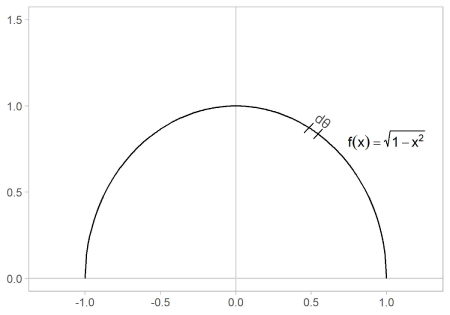
\includegraphics[scale=0.6]{img/avg-val-ex-2.jpg}
\end{figure}

La longitud de arco $s$ se calcula como $s = \theta \cdot r$, donde $\theta$ es el ángulo en radianes tomado desde el centro de un círculo y $r$ es su radio. Como estamos trabajando con un semicírculo unitario, entonces $s = \theta$. Si, por ejemplo, dividimos el arco desde $\theta = 0$ en tres partes, de largo $s = \pi/6$, sus distancias serán ese mismo valor:
\[
  \left|\frac{\pi}{6} - 0\right| =
  \left|\frac{2\pi}{6} - \frac{\pi}{6}\right| = 
  \left|\frac{3\pi}{6} - \frac{2\pi}{6}\right| = \frac{\pi}{6}
\]
No obstante, cuando calculamos las mismas distancias con respecto a $x$, éstas no son iguales.
\[
  \left|\cos\left(\frac{\pi}{6}\right) - \cos(0)\right| \neq
  \left|\cos\left(\frac{2\pi}{6}\right) - \cos\left(\frac{\pi}{6}\right)\right| \neq
  \left|\cos\left(\frac{2\pi}{6}\right) - \cos\left(\frac{\pi}{6}\right)\right|
\]
Lo anterior explica por qué la altura promedio que calcularemos acá será distinta a la del ejercicio anterior.

Cuando trabajamos en relación a $\theta$ en un (semi)círculo unitario, la distancia vertical es $y = \sin(\theta) - 0 = \sin(\theta)$, con $y = f(x)$. En cuanto a la altura promedio calculada a partir del valor promedio continuo, estará en el intervalo $[0, \ \pi]$. Con todo, resulta en:
\[
  \frac{1}{\pi - 0} \cdot \int_{0}^{\pi} \sin(\theta) d\theta = \frac{1}{\pi} \cdot [-\cos(\theta)]_{0}^{\pi} = \frac{2}{\pi}
\]
y veamos que
\[
  \frac{1}{2} \cdot \int_{-1}^{1} \sqrt{1 - x^{2}}dx  > \frac{1}{\pi} \cdot \int_{0}^{\pi} \sin(\theta) d\theta 
\]
aunque ambos son las alturas promedios del semicírculo unitario, pero medidos con respecto a distintas variables.

\subsection{Promedio Ponderado.}

En ciertas ocasiones queremos calcular el promedio de una cantidad determinada de valores, pero en su contexto algunos tienen mayor relevancia que otros. En esos casos conviene usar el \textbf{promedio ponderado}, el cual se calcula como:
\[
  \frac{\sum_{i = 1}^{n} f(x_{i}) \cdot w(x_{i})}{\sum_{i = 1}^{n} w(x_{i})}
\]
donde $w(x_{i})$ es el valor que le dará el ``peso'' o relevancia relativa a cada $f(x_{i})$.

\textbf{Ejemplo.} En la siguiente tabla se encuentran las notas que obtuvo una estudiante en un curso, cada una con una ponderación distinta. Calcule su promedio final.

\begin{table}[hbt!]
\centering

\begin{tabular}{c|c c c c}
Notas & $6.7$ & $6.2$ & $5.0$ & $4.2$ \\
\hline
Porcentaje & $20\%$ & $30\%$ & $30\%$ & $20\%$
\end{tabular}

\end{table}

\textbf{Solución.} En este ejemplo nos piden calcular el promedio ponderado. Acá es mejor trabajar los porcentajes como decimales. Por lo tanto, el promedio final que obtuvo la estudiante es el siguiente:
\[
  \frac{(6.7 \cdot 0.2) + (6.2 \cdot 0.3) + (5.0 \cdot 0.3) + (4.2 \cdot 0.2)}{0.2 + 0.3 + 0.3 + 0.2} = \frac{5.54}{1} = 5.54
\]

Si $n \to \infty$ en el promedio ponderado, obtenemos su versión \textbf{continua}:
\[
  \lim_{n \to \infty} \left(\frac{\sum_{i = 1}^{n} f(x_{i}) \cdot w(x_{i})}{\sum_{i = 1}^{n} w(x_{i})}\right) =
  \frac{\int_{a}^{b} f(x)w(x) dx}{\int_{a}^{b} w(x)dx}
\]

\subsection{Agua hervida en una caldera.}

Al final de la clase anterior calculamos el volumen de $1$m de alto y $2$m de ancho, que fue de $\approx 1571$ Lt. Ahora la volveremos a usar para el siguiente ejemplo:

\textbf{Ejercicio 3.} Suponga que quiere hervir agua adentro de una caldera. Sin alguna fuente de calor, la temperatura inicial $T_{0}$ se mantiene a la del ambiente, que es de $0^{\circ}$C.

Al encender una hoguera abajo de la caldera, la temperatura final del agua $T_{F}$ varía linealmente en función de la altura $h$ del contenedor como $T_{F} = (100 - 30h)^{\circ}$C. Es decir, en el fondo de ella, $T_{F} = 100^{\circ}$C y en la parte alta, $T_{F} = 70^{\circ}$C.

\begin{figure}[hbt!]
\centering
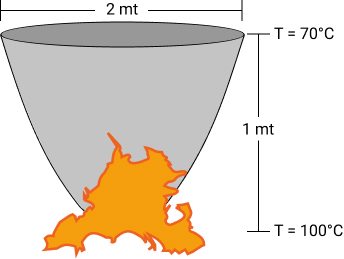
\includegraphics[scale=0.45]{img/cauldron-heat-1.jpg}
\end{figure}

Calcule la cantidad de energía necesaria para llevar el agua a su punto de ebullición a partir de la fórmula $E = T_{F} \cdot V$, donde $E$ es la energía y $V$ el volumen de la caldera.

\textbf{Solución.} Para obtener la energía $E$, necesitamos calcular el volumen de la caldera y, para ello, podemos ``rebanarla'' usando uno de los métodos de los sólidos de revolución visto en la clase anterior.

La caldera podemos modelarla como una parábola $f(x) = x^{2}$ siendo girada desde su mitad $x \geq 0$ alrededor de $y = f(x)$.

Como la temperatura adentro de la caldera varía con respecto a su altura, la mejor opción es dividir la parábola de forma horizontal, porque se mantendrá constante en cada nivel vertical.

%\newpage

\begin{figure}[hbt!]
\centering
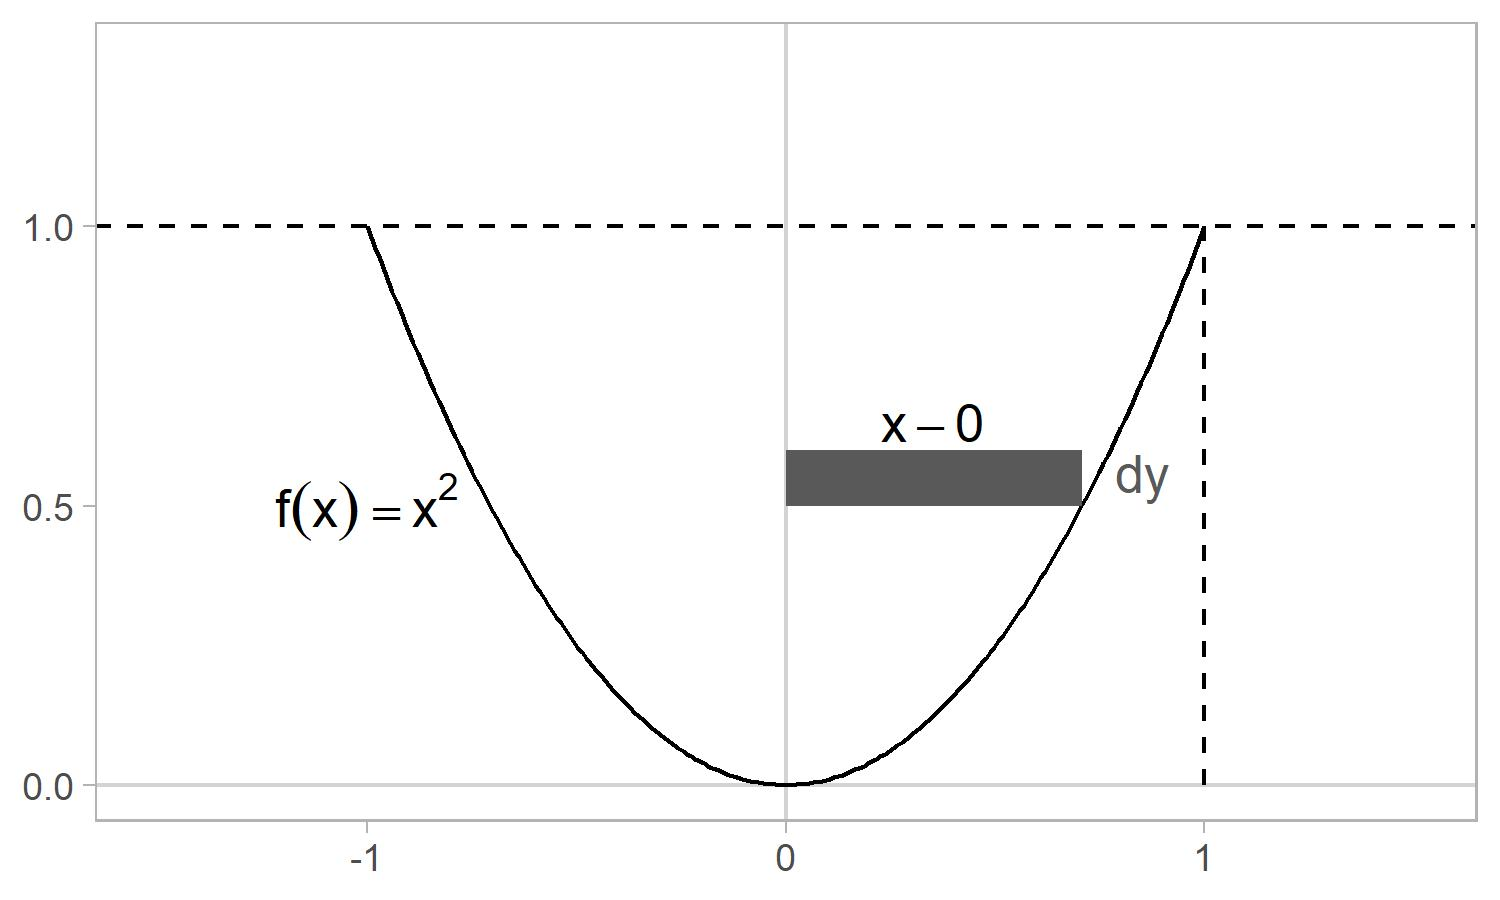
\includegraphics[scale=0.55]{img/cauldron-heat-2.jpg}
\end{figure}

Al hacer girar la mitad $x \geq 0$ de la parábola, el rectángulo que vemos en el gráfico de arriba pasará a ser un \textbf{disco}, de manera que podemos usar el volumen de este sólido para calcular el de la caldera, donde el radio de su sección transversal es el largo de la figura inicial y no olvidemos que lo estamos haciendo con respecto a $y$.
\[
  V = (\pi r^{2}) \Delta y = (\pi x^{2}) \Delta y
\]
Y no olvidemos que estamos generando el disco con respecto a $y$, donde $y = x^{2}$
\[
  V = (\pi y) \Delta y
\]
Así, la energía necesaria final $E_{F}$ podemos calcularla como la suma acumulada de las energías de cada rebanada de la caldera, entre $0 \leq y \leq 1$. Veamos que su altura $h = y$ en la parábola.
\[
  E_{F} = \int_{0}^{1} Edy
        = \int_{0}^{1} [T_{F} \cdot V]dy
        = \int_{0}^{1} [(100 - 30y) \cdot (\pi y)]dy
        = \pi \cdot \left[\frac{100y^{2}}{2} - \frac{30y^{3}}{3}\right]_{0}^{1}
        = 40 \pi
        \approx 126
\]
Por lo tanto, la cantidad de energía necesaria para hervir el agua adentro de la caldera, es de $\approx 126^{\circ} \text{C} (\text{m}^{3})$.

\textbf{Ejercicio 4.} Calcule la temperatura final promedio que alcanza el agua adentro de la caldera cuando la hoguera ya está encendida.

\textbf{Solución.} En el ejercicio anterior, vimos que en la energía necesaria para hervir el agua en la caldera, la temperatura final (que está en función de su altura) es amplificada o disminuida por el volumen del contenedor. Por lo tanto, la temperatura promedio, que denotaremos como $T_{P}$ estará ponderada por dicha medida.
\[
  T_{P} = \frac{\int_{0}^{1} [(100 - 30y) \cdot (\pi y)] dy}{\int_{0}^{1} (\pi y) dy}
\]
El numerador lo calculamos en el ejercicio previo, que fue igual a $(40 \pi)^{\circ} \text{C} \cdot \text{m}^{3}$. En cuanto al denominador, lo obtuvimos en la clase pasada, pero ahí usamos el método del caparazón cilíndrico. Con el de los discos (el usado acá) deberíamos obtener el mismo resultado: $(\pi/2) \text{ m}^{3}$.
\[
  \int_{0}^{1} (\pi y)dy = \pi \cdot \left[\frac{y^{2}}{2}\right]_{0}^{1} = \frac{\pi}{2} \text{ m}^{3}
\]
Por lo tanto, la temperatura final ponderada la calculamos como:
\[
  T_{P} = \frac{\int_{0}^{1} [(100 - 30y) \cdot (\pi y)] dy}{\int_{0}^{1} (\pi y) dy}
        = \frac{40 \pi}{(\pi/2)}
        = 80^{\circ} \text{C}
\]


\section{Probabilidades.}

Posiblemente hemos estudiado que la \textbf{probabilidad de un evento} $A$, $P(A)$, lo calculamos como la proporción:
\[
  P(A) = \frac{\text{Parte}}{\text{Todo}}
\]
Esta proporción también podemos interpretarla como un \textbf{promedio ponderado}. Recordemos que cuando es continuo, lo calculamos como:
\[
  \frac{\int_{a}^{b} f(x)w(x) dx}{\int_{a}^{b} w(x)dx}
\]
Acá $f(x)$ es constante y toma los números $1$ o $0$, según si la integral es calculada adentro o no del área del evento. Como el propósito es siempre conocer el primer caso, entonces $f(x) = 1$. Mientras que $w(x)$ es la que refleja la proporción del área con respecto al total.

Así, la probabilidad de un evento se define como sigue:

\textbf{Definición.} Si tomamos aleatoriamente un punto entre $a \leq x_{1} < x_{2} \leq b$, la probabilidad de que esté adentro de ese intervalo, $P(x_{1} < x < x_{2})$, se calcula como:
\[
  P(x_{1} < x < x_{2}) = \frac{\int_{x_{1}}^{x_{2}} w(x)dx}{\int_{a}^{b} w(x)dx}
\]
\textbf{Ejemplo 2.} Suponga que toma un punto $(x, \ y)$ ``aleatoriamente'' del intervalo $0 < y < 1-x^{2}$. Calcule la probabilidad de que $x$ de dicho punto sea mayor a $1/2$.

\begin{figure}[hbt!]
\centering
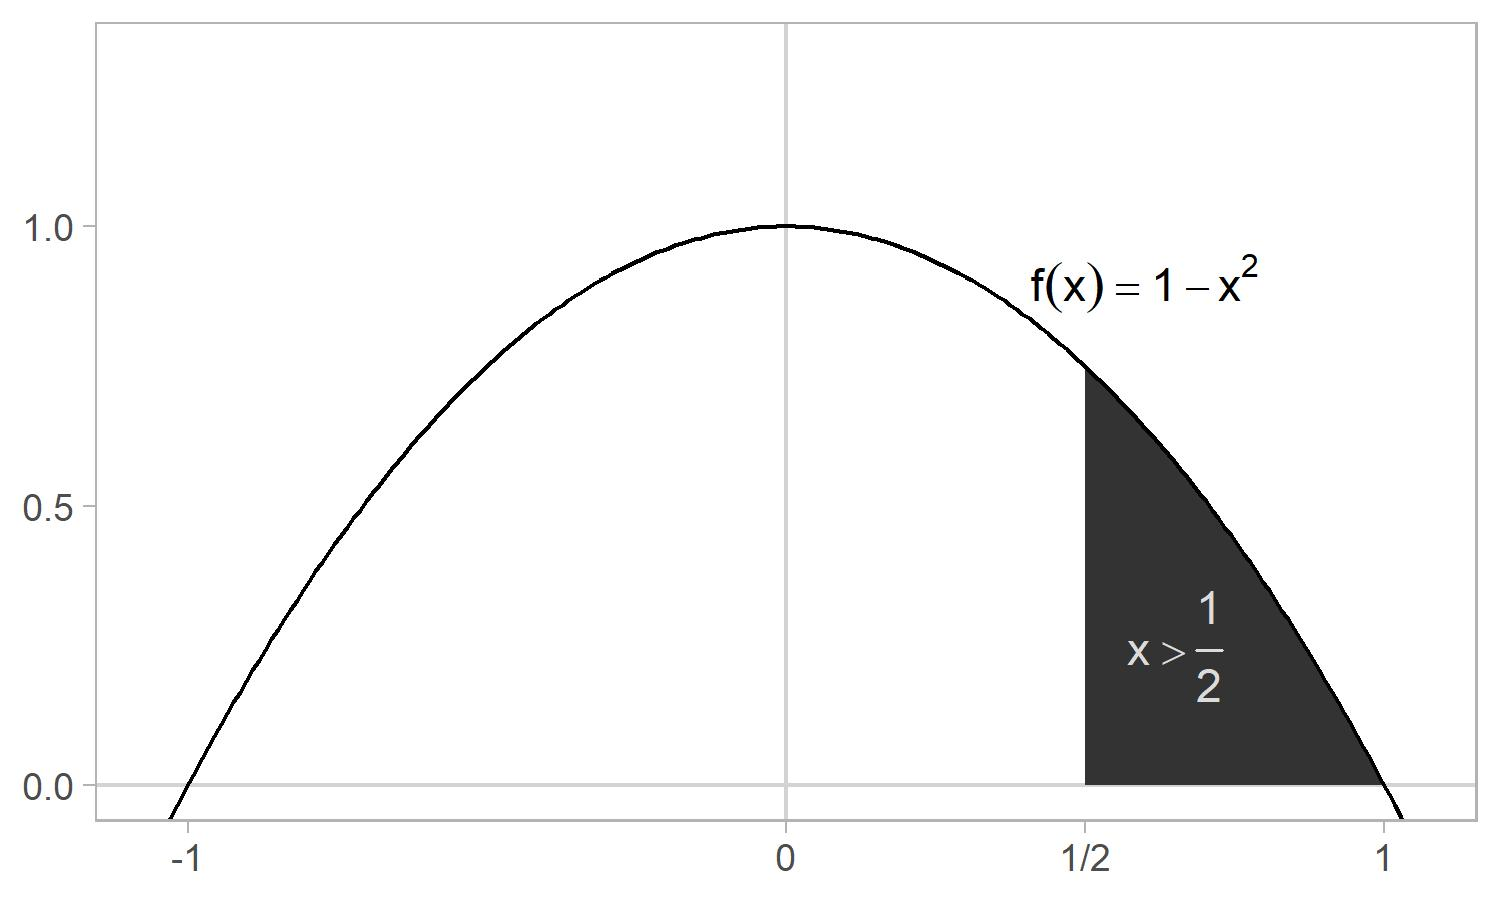
\includegraphics[scale=0.55]{img/prob-example.jpg}
\end{figure}

\textbf{Solución.} Cuando nos dicen que tomamos un punto adentro del intervalo $(0, \ 1-x^{2})$ en $y$, quiere decir que es bajo la curva $f(x) = 1 - x^{2}$, donde $y = f(x)$, y sobre la recta $y = 0$. Por lo tanto, la probabilidad será el cociente entre el área bajo $f(x)$ para todo $1/2 < x < 1$ y el área total.
\[
  P\left(\frac{1}{2} < x < 1\right) = \frac{\int_{1/2}^{1} [1 \cdot (1 - x^{2})]dx}{\int_{-1}^{1} (1 - x^{2})dx}
                                    = \frac{\int_{1/2}^{1} (1 - x^{2})dx}{\int_{-1}^{1} (1 - x^{2})dx}
\]
Para mayor legibilidad, calcularemos las integrales de forma separada:
\begin{align*}
\int_{1/2}^{1} (1 - x^{2})dx &= 1 - \left[\frac{x^{3}}{3}\right]_{1/2}^{1} &
\int_{-1}^{1} (1 - x^{2})dx &= 1 - \left[\frac{x^{3}}{3}\right]_{-1}^{1} \\
&= \frac{5}{24} &
&= \frac{4}{3}
\end{align*}
Por lo tanto:
\[
  P\left(\frac{1}{2} < x < 1\right) = \frac{\int_{1/2}^{1} (1 - x^{2})dx}{\int_{-1}^{1} (1 - x^{2})dx}
                                    = \frac{5/24}{4/3}
                                    = \frac{5}{32}
                                \approx 0.17
\]

\end{document}
